% Use class option [extendedabs] to prepare the 1-page extended abstract.
\documentclass[extendedabs]{bmvc2k}
\usepackage[colorlinks = true,
            linkcolor = blue,
            urlcolor  = blue,
            citecolor = blue,
            anchorcolor = blue]{hyperref}
\usepackage{kotex}
% for the fancy \koTeX logo
\usepackage{kotex-logo}
\usepackage{mathtools}  % brings in amsmath, also some improvements
\usepackage{amssymb} % brings in amsfonts, incl \square
% Document starts here
\begin{document}


\title{Faster R-CNN pre-report}
\addauthor{
Taehun Kim$^{1}$
}{}{1}

\addinstitution{
$^1$ Department of Computer Science and Engineering, Pusan National University.  
}
 

\maketitle
\noindent


\begin{figure}[t]
	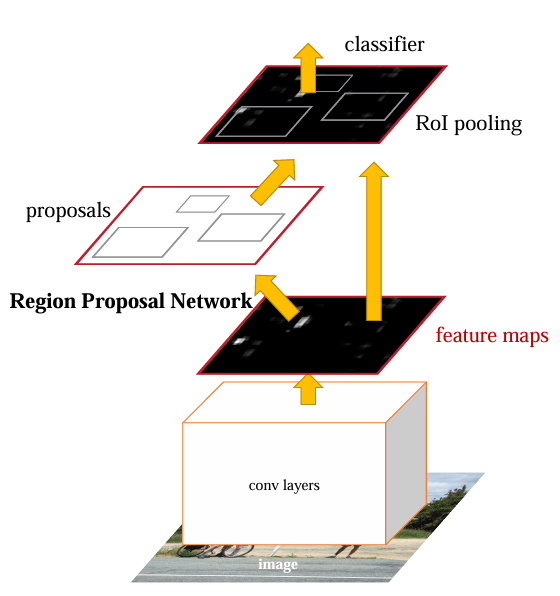
\includegraphics[width=\linewidth]{images/fasterrcnnarch.PNG}
	\caption{
		The architecture of Fast R-CNN\cite{fasterrcnn}}
	\vspace{-2mm}
 \label{fig:fasterrcnnarch}
\end{figure}





\section{Introduction}
Faster R-CNN\cite{fasterrcnn} is an object detection network that generates region proposals using a deep convolutional network. the deep convolutional network is called \textit{Region Proposal Networks}. This method reduces the computational cost of generating proposals while improving accuracy.

In this report, We implement Faster R-CNN\cite{fasterrcnn},  train the model using recyclable photo data, locate recyclable objects in images, and classify their classes.
\section{Dataset}
We use recyclables images data of NAVER Connect Foundation boostcamp AI Tech. There are 4883 training images and 4871 testing images. The size of the images is $1024\times1024$. There are 10 classes, which are General trash, Paper, Paper pack, Metal, Glass, Plastic, Styrofoam, Plastic bag, Battery, Clothing.
\subsection{Data augmentation}
With 4,883 training images, the dataset may be insufficient for training. Therefore, we augment the training images using the Albumentations library. This library provides tools for image data augmentation and automatically adjusts bounding box positions during transformations. We flip, change brightness, change contrast, change hue and saturation with 50\% probability for augmentation.
\section{Shared convolutional network}
We use a pretrained VGG-16 network with fully connected layers and dropout removed for feature extraction. Additionally, we freeze the first 10 layers, allowing only the last 4 layers to be trainable. This prevents the pre-trained weight from being over-fitted.
\section{Region Proposals Network}
The shape of the last feature map of the VGG-16 network is $(64,64,512)$. And we applied $3\times3$ convolutional layer with padding to this feature map. The role of this layer is a sliding window, mapping a $3\times3\times512$ to a lower-dimensional $1\times1\times512$ feature map. The lower-dimensional feature map is fed to two $1\times1$ convolutional layers. one is a box coordinate regression layer, and the other is a box classification layer. The output of box coordinate layer are transform to currect the anchors\ref{anchor}. the output of box regression layer are the probability of whether there is an object in the box or not.
\subsection{Anchors} \label{anchor}
At center of each sliding-window location, We predict multiple region proposals. We predict 9 proposals per sliding window in this lab. The 9 proposals are relative to k reference boxes, which is called \textit{anchors}. this means that the 9 proposals is calculated using anchors and box coordinate regression layer. Therefore, box coordinate regression layer's output channel is $36(=9\times4)$, and box classification layer's output channel is $18(=9\times2)$.

In this lab, we generate 9 anchor boxes. The base size is $(16\times16)$, ratios are 0.5,1 and 2, scales are 8,16 and 32. In other words, we generate 9 anchors box with 3 different sizes(128, 256, 512) and 3 different ratios(0.5, 1, 2). Since the shape of the feature map is $64\times64\times512$, a total of $36864(=64\times64\times9)$ anchors are generated per image. Note that the size of anchor boxes are related to the original image.

\subsection{Region of Interests}
We generate the Region of Intertests(RoI) to be input to the head(classifier in \ref{fig:fasterrcnnarch} using the anchors and RPN's output.

First, we calculate the RoI using the following formula\cite{rcnn}:
$$
b_x = p_x + p_wt_x
$$
$$
b_y = p_y + p_ht_y
$$
$$
b_w = p_we^{t_w}
$$
$$
b_h = p_he^{t_h}
$$
where b is RoI bounding box, p is anchors, t is output of box coordinate layer. Also, (x,y) is center coordinate of boxes, w is width, and h is height.

Second, we clip region proposals to stay within the image boundaries. Third, we removed region proposals smaller than 16 in size. Fourth, we selected the top 12000(6000 in test) region proposals based on the box classification score. Finally, we adopt non-maximum suppression(NMS) on the region proposals. We fix the IoU threshold at 0.7, and we selected the top 2000(300 in test) region proposals after NMS.
\section{RoIHead Network}
The RoIHead network is final part of the Faster R-CNN\cite{fasterrcnn}. This network is responsible for classifying objects and refining bounding boxes in the RoI generated by RPN. This network takes the RoI as input, perform RoI pooling\cite{fastrcnn}. RoI pooling applies max pooling to each RoI to generate fixed $(7\times7)$ feature maps, regardless of the original size.

These features are fed to classifier network, which is extracted from first two fully-connected layers of pre-trained VGG-16. Also, Output of the last classifier layer is fed to two fully-connected layers, one is bounding box regression layer and another is box classification layer. Note that this box classification layer classify the type of the object.
\section{Training}
We trained the model with 0.0001 learning rate, 0.0005 weight decay and 14 epochs. Additionally, we reduce the learning rate by a factor of 10 after 9 epochs. box regression loss is smooth L1 loss\cite{fastrcnn}, and box classification loss is softmax cross entropy loss. The box regression loss is calculated only for positive anchors.

\subsection{Anchor Target}
For training RPNs, We assign binary class label to each anchor. We assign a positive(=1) label to two kinds of anchors: one is the anchor with the highest IoU overlap with the ground-truth box, and another is anchor that has an IoU higher than 0.7 with any ground-truth box. The first condition is adopted because some ground-truth boxes may not have corresponding positive anchors. 

We assign a negative label(=0) to a anchor that IoU ratio is lower than 0.3 for all ground-truth boxes.

The box regression target is the offset($t_y,t_x$) and scale difference($t_w,t_h$) between an anchor and the ground-truth box with the highest IoU with that anchor:

$$
t_x = (b_x-p_x)/p_w
$$
$$
t_y = (b_y-p_y)/p_h
$$
$$
t_w = log(b_w/p_w)
$$
$$
t_h = log(b_h/p_h)
$$

If there are more than 128 positive or negative anchors, only 128 of each are used for loss function through random sampling.
\subsection{Proposal Target}
For training head network(Fast R-CNN network), We assign the target class for the proposal as the class label of the ground-truth box with the highest IoU with that Region Proposal. We also set the target box coordinates as the offset and scale difference between a proposal and the ground-truth box with the highest IoU for that anchor. 

We assign a positive label to a anchor that highest IoU is equal or bigger than 0.5, and we assign a negative label to a anchor that highest IoU is less than 0.5. Then, through random sampling, 35 positive proposals and 93 negative proposals are selected for use in the loss function.
\section{Result and Inference}
\begin{figure}[thb] \centering
    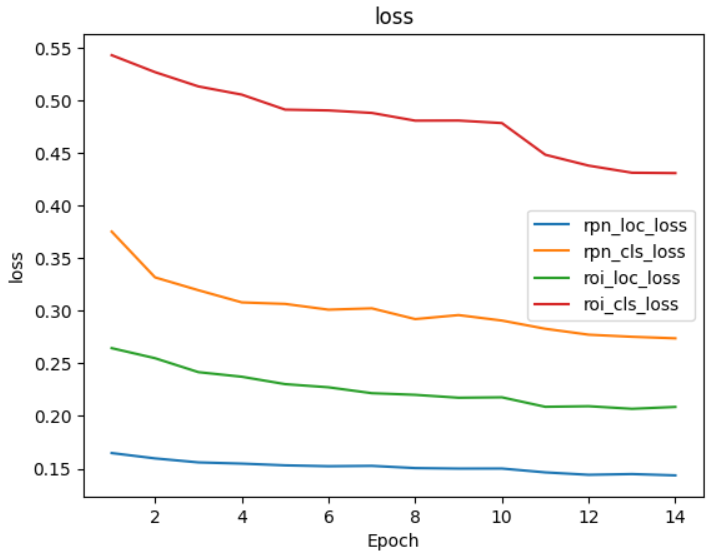
\includegraphics[width=0.23\textwidth]{images/train loss.PNG}
    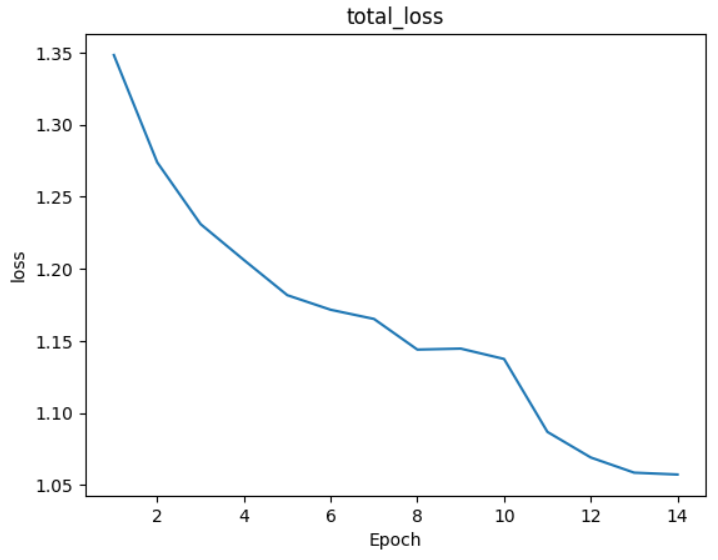
\includegraphics[width=0.23\textwidth]{images/total loss.PNG}
    \caption{each train loss(left) and total train loss(right)} \label{fig:figure2}
\end{figure}
The losses after last epoch are on table \ref{tab:losstable}. The total loss after last epoch is 1.057. The training seems to have gone well because each loss is less than 0.5.

We inference object bounding boxes and classification of test images using trained model. The inferred bounding boxes and classes were saved in a CSV file. Since there are no target bounding boxes or class labels, we cannot calculate the mAP.

The inference time for 4,871 test images was 5 minutes and 59 seconds (359 seconds) on an A5000 GPU, indicating that it took approximately 0.074 seconds to infer a single image. This corresponds to a processing rate of about 13.57 images per second (13.57 FPS).

\section{Conclusion}
We implemented Faster R-CNN\cite{fasterrcnn} and we train the model with recyclables images. We then infer the bounding boxes and classifications of the objects in the test images. The inference rate is about 13.57 FPS on A5000 GPU. This recyclables object detection model could potentially be used in robots or recycling facilities.

\begin{table}[]
\centering
\begin{tabular}{|l|l|}
\hline
               & loss  \\ \hline
rpn\_loc\_loss & 0.144 \\ \hline
rpn\_cls\_loss & 0.274 \\ \hline
roi\_loc\_loss & 0.209 \\ \hline
roi\_cls\_loss & 0.431 \\ \hline
total loss     & 1.057 \\ \hline
\end{tabular}
\caption{The losses after last epoch. rpn is RPN network, roi is head network. loc is bounding box regression, loc is bounding box classification. Each value was rounded to three decimal places.}
\label{tab:losstable}
\end{table}
\newpage
\bibliography{egbib}

\end{document}
